\documentclass[10pt,a4paper]{scrartcl}
\usepackage[utf8]{inputenc}
\usepackage{lmodern}
\usepackage[intlimits]{amsmath}
\usepackage[hidelinks=true]{hyperref}
\usepackage{url}
\usepackage{breakurl}
\usepackage{booktabs}
\usepackage{amsfonts}
\usepackage{amssymb}
\usepackage{graphicx}
\usepackage{todonotes}
\usepackage{enumerate} 
\usepackage{bm} 
\usepackage{physics} 
\usepackage{cleveref} 
\usepackage{pgfplots} 

\newcommand{\ve}[1]{\bm{#1}} 
\newcommand{\Dv}[2]{\frac{\mathrm{D}#1}{\mathrm{D}#2}} 

\newcounter{problemcounter}

\newenvironment{problem}{%
\refstepcounter{problemcounter}%
\noindent%
\textbf{Problem \theproblemcounter:} }{}

\usepackage[separate-uncertainty=true, exponent-product=\cdot]{siunitx}
\begin{document}
\title{\Huge Submission 1}
\author{Philipp Stärk}
\date{\small \today}
\maketitle

\begin{problem}
Self avoiding polymer model:

\begin{enumerate}[a)]
\item Probability distribution of 4 monomer chain:

Possible values for chain length (found by Drawing): $ |\ve{R}_3 - \ve{R}_0| = 1, \sqrt{5}, 3 $.

Probabilities, determined by enumeration and symmetry arguments:
    \begin{table}[h]
        \centering
        \begin{tabular}{@{}ll@{}}
            \toprule
            $ p $ & Value\\\midrule
            $ p (|\ve{R}_3 - \ve{R}_0| = 1) $ & $\frac{2}{9}$ \\
            $ p (|\ve{R}_3 - \ve{R}_0| = \sqrt{5}) $ & $\frac{6}{9}$ \\
            $ p (|\ve{R}_3 - \ve{R}_0| = 3) $ & $ \frac{1}{9}  $ \\\bottomrule
        \end{tabular} 
    \end{table}

    The probability to find the chain in a straight line is that of $ p(|\ve{R}_3 - \ve{R}_0| = 3) = \frac{1}{9} $.

\item Mean:
    \begin{equation*}
        \expval{\abs{\ve{R}_3 - \ve{R}_0}} = \frac{2}{9} + \sqrt{5} \frac{6}{9} + 3 \frac{1}{9} \approx 2.04
    \end{equation*}

    Variance:
    \begin{equation*}
        \sigma = \sqrt{\expval{\abs{ \ve{R}_3 - \ve{R}_0}^2}} = \sqrt{ \frac{2}{9} + 5 \frac{6}{9} + 9 \frac{1}{9}  } \approx 1.91
    \end{equation*}
\end{enumerate}
\end{problem}

\begin{problem}
Random walk on a lattice without self-avoidance:

\begin{enumerate}[a)]
\item \label{it:a} Probability distribution $ p (X, Y | N) $:

Start with considering random walk in $ x $-direction, assume $ N_x = r + l$ steps in this direction, with $ r $ the steps in positive and $ l $ steps in negative direction, i.e.\  $ X = r - l $.

$ \implies r-l =x, N = r+l \implies r = \frac{N_x + x}{2}, l = \frac{N_x - x}{2} $.

Thus, we have
\begin{equation*}
    p(X|N_x) = \begin{pmatrix}N_x\\\frac{N_x + x}{2}\end{pmatrix} p^{N_x}
\end{equation*}
in one direction (of course analogously in $ y $-direction), with $ p = \frac{1}{2}  $.

To get the probability $ p(X, Y|N) $, we need to sum over all combinations of possible number of path-steps in each direction, where we know:
\begin{gather*}
    N = N_x + N_y,\\
    \forall N_x \in \{ X, \dots,  N-Y \},\\
    \forall N_y \in \{ Y, \dots,  N-X \}.\\
\end{gather*}

Thus, overall, we have:
\begin{equation*}
    p(X, Y|N) = \sum _{N_x = X}^{N-Y} \begin{pmatrix}N_x\\ \frac{N_x + X}{2}\end{pmatrix} \begin{pmatrix}N - N_x\\ \frac{N - N_x + Y}{2}  \end{pmatrix} \frac{1}{4}^N,
\end{equation*}
with the condition that $ X + Y $ is even (odd), if $ N $ is even (odd), otherwise we immediately know $ p(X, Y|N) = 0 $, because there is no possible path to that point.

I am not sure if there is a more elegant, close form solution to this probability distribution, because this is a bit ugly.

\item\label{it:b} Mean value:

    One can reason that there is nothing special about the $ x $-direction, i.e. $ \expval{N_x} = \frac{N}{2} $, thus, we may use the probability distribution $ p(X|N_x) $ as defined above in \ref{it:a}).
\begin{equation*}
    \expval{X|N} = \sum_{X} X p(X|\underbrace{N_x}_{= N/2}) = \sum_{X=0}^{N} X \begin{pmatrix}
        N/2\\ \frac{N/2 + X}{2}
    \end{pmatrix} \frac{1}{2}^{N/2}
\end{equation*}
The same obviously holds for $ \expval{Y|N} $.

\item The path cannot return to (0,0) for odd number of jumps, as $ X + Y = 2\mathbb{N} $ is only possible for even numbers of steps.

The probability function: for a return to the starting point can be determined like this: Consider that to end up at the same square one has to walk $ r  $ steps to the right and $ l = r $ steps to the left.
Similarly, one has to walk the same number of steps upwards compared to downwards.
Again, there is nothing special about each directions, so this will be the probability of one walker coming back to zero squared, with the average number of steps in one direction being $ n := N/2 $:
\begin{equation*}
    p (0, 0| \underbrace{2n}_{=N}) = \left(  \begin{pmatrix}2n\\ n \end{pmatrix} \frac{1}{2^{2n}} \right)^2.
\end{equation*}

To see the asymptotic behavior of this formula, confer with fig.~\ref{fig:asymptote}.
\begin{figure}[h]
    \centering
    % This file was created by tikzplotlib v0.9.2.
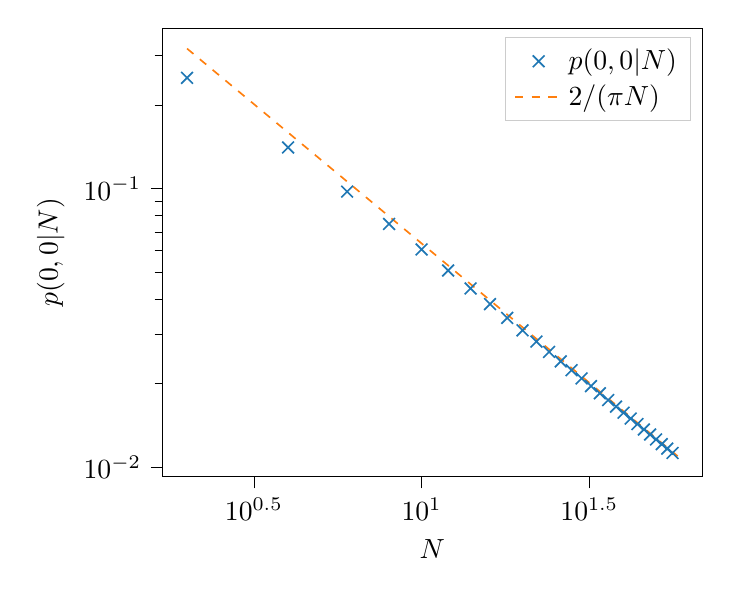
\begin{tikzpicture}

\definecolor{color0}{rgb}{0.12156862745098,0.466666666666667,0.705882352941177}
\definecolor{color1}{rgb}{1,0.498039215686275,0.0549019607843137}

\begin{axis}[
legend cell align={left},
legend style={fill opacity=0.8, draw opacity=1, text opacity=1, draw=white!80!black},
log basis x={10},
log basis y={10},
tick align=outside,
tick pos=left,
x grid style={white!69.0196078431373!black},
xlabel={\(\displaystyle N\)},
xmin=1.69009102606365, xmax=68.635356445962,
xmode=log,
xtick style={color=black},
y grid style={white!69.0196078431373!black},
ylabel={\(\displaystyle p(0, 0|N)\)},
ymin=0.0092753910714925, ymax=0.376677801698243,
ymode=log,
ytick style={color=black}
]
\addplot [semithick, color0, mark=x, mark size=3, mark options={solid}, only marks]
table {%
2 0.25
4 0.140625
6 0.09765625
8 0.07476806640625
10 0.0605621337890625
12 0.0508890151977539
14 0.0438787937164307
16 0.0385653460398316
18 0.0343993364367634
20 0.031045401134179
22 0.0282872353309358
24 0.0259790755035851
26 0.0240191156652969
28 0.0223341011734712
30 0.0208699767632103
32 0.0195859840521925
34 0.0184508102360187
36 0.0174400019591998
38 0.0165341846829256
40 0.0157178093142061
42 0.0149782525267463
44 0.014305159567125
46 0.01368995658007
48 0.0131254835439994
50 0.012605714395657
52 0.0121255411032189
54 0.0116806052671268
56 0.0112671654761029
};
\addlegendentry{$p(0,0|N)$}
\addplot [semithick, color1, dashed]
table {%
2 0.318309886183791
3.14285714285714 0.202560836662412
4.28571428571429 0.148544613552436
5.42857142857143 0.11727206333087
6.57142857142857 0.0968769218820233
7.71428571428571 0.0825247853069087
8.85714285714286 0.0718764259124689
10 0.0636619772367581
11.1428571428571 0.0571325436740137
12.2857142857143 0.0518178884485241
13.4285714285714 0.0474078553890752
14.5714285714286 0.0436895922213046
15.7142857142857 0.0405121673324825
16.8571428571429 0.0377655797167209
18 0.0353677651315323
19.1428571428571 0.0332562567654707
20.2857142857143 0.0313826648350216
21.4285714285714 0.0297089227104871
22.5714285714286 0.0282046734593232
23.7142857142857 0.0268454120877896
24.8571428571429 0.0256111402676613
26 0.0244853758602916
27.1428571428571 0.0234544126661741
28.2857142857143 0.0225067596291569
29.4285714285714 0.0216327107115198
30.5714285714286 0.0208240112456686
31.7142857142857 0.0200735964260048
32.8571428571429 0.0193753843764047
34 0.0187241109519877
35.1428571428571 0.0181151967746873
36.2857142857143 0.017544639395957
37.4285714285714 0.0170089252159277
38.5714285714286 0.0165049570613817
39.7142857142857 0.0160299942682485
40.8571428571429 0.0155816028201856
42 0.0151576136277996
43.1428571428571 0.0147560874389837
44.2857142857143 0.0143752851824938
45.4285714285714 0.0140136427879656
46.5714285714286 0.0136697497134143
47.7142857142857 0.013342330558602
48.8571428571429 0.0130302292589856
50 0.0127323954473516
51.1428571428571 0.0124478726440589
52.2857142857143 0.0121757879961013
53.4285714285714 0.0119153433330831
54.5714285714286 0.0116658073470499
55.7142857142857 0.0114265087348027
56.8571428571429 0.011196830167269
58 0.0109762029718549
};
\addlegendentry{$2/(\pi N)$}
\end{axis}

\end{tikzpicture}

    \caption{Exact probability for $ p(0,0|N) $ plotted together with $ 2/(\pi N) $.}
    \label{fig:asymptote}
\end{figure}

\item To prove the asymptotic behavior of this random walk, start with the probability function as above
 \begin{equation*}
     p (0, 0| N) = \left(  \begin{pmatrix}N\\ N/2 \end{pmatrix} \frac{1}{2^{2n}} \right)^2 = \left(\frac{N!}{(N/2)!(N - N/2)!} \frac{1}{2^N}\right)^2 = \left(\frac{N!}{((N/2)!)^2} \frac{1}{2^N}\right)^2
 \end{equation*}
 Using Stirling's approximation $ n! \to \sqrt{2\pi n} (n/e)^n (n \to \infty)$, we have
 \begin{gather*}
     p(0,0|N) \to \left(\frac{\sqrt{2\pi N}(N/e)^N}{(\sqrt{\pi N} (N/2e)^{N/2})^2} \frac{1}{2^N}\right)^2   \qquad(N \to \infty)\\
     \to \left( \frac{\sqrt{2}}{\sqrt{\pi N}} \frac{2^N}{2^N} \right)^2 = \frac{2}{\pi N}.
 \end{gather*}
\end{enumerate}
\end{problem}

\end{document}
